\begin{figure}[t]
    \centering
    \begin{subfigure}[b]{.24\linewidth}
        \centering
        \resizebox{\linewidth}{!}{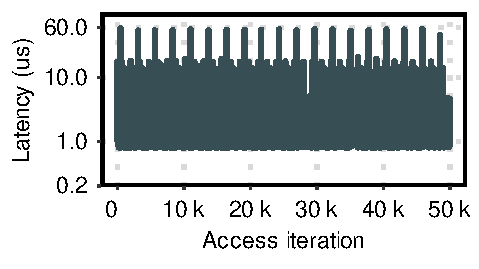
\includegraphics{figure/plot/reference/fig5a-overwrite-iter-lat.pdf}}
        \caption{\label{fig:5a:refoverwrite-iter-latency}[Ref]Per-iter latency.}
    \end{subfigure}
    \hfill
    \begin{subfigure}[b]{.24\linewidth}
        \centering
        \resizebox{\linewidth}{!}{\includegraphics{example-image-duck}}
        % \includegraphics[width=\linewidth]{}
        \caption{\label{fig:5b:ref:overwrite-delay-p99-latency-sample}[Ref]99.99 percentile latencies.}
    \end{subfigure}
    \hfill
    \begin{subfigure}[b]{.24\linewidth}
        \centering
        \resizebox{\linewidth}{!}{\includegraphics{example-image-duck}}
        % \includegraphics[width=\linewidth]{}
        \caption{\label{fig:5a:repoverwrite-iter-latency}[Rep]Per-iter latency.}
    \end{subfigure}
    \hfill
    \begin{subfigure}[b]{.24\linewidth}
        \centering
        \resizebox{\linewidth}{!}{\includegraphics{example-image-duck}}
        % \includegraphics[width=\linewidth]{}
        \caption{\label{fig:5b:rep:overwrite-delay-p99-latency-sample}[Rep]99.99 percentile latencies.}
    \end{subfigure}

    \caption{\label{fig:5:overwrite}Overwrite microbenchmark results.}
\end{figure}
